\documentclass[11pt]{overturerep} \usepackage{t1enc,times,a4,t1enc}
\usepackage{graphicx}

\usepackage{listings} \usepackage{times} \usepackage{color}
\usepackage[bookmarks]{hyperref} \lstdefinelanguage{VDM++}
  {morekeywords={act, active, fin, req, waiting, abs, all, allsuper, always, and, answer, 
     assumption, async, atomic, be, bool, by, card, cases, char, class, comp, compose, conc, cycles,
     dcl, def, definitions, del, dinter, div, dlmodule, do, dom, dunion, duration, effect, elems, else, elseif, end,
     error, errs, exists, exists1, exit, exports, ext, floor, for, forall, from, functions, 
     general, hd, if, imports, in, inds, infer, init, inmap, input, instance, int, inter, inv, inverse, iota, is, 
     isofbaseclass, isofclass, inv, inverse, lambda, len, let, map, measure, mu,
     mutex, mod, module, nat, nat1, new, merge, 
     munion, not, of, operations, or, others, per, periodic, post, power, pre, pref, 
     private, protected, public, qsync, rd, responsibility, return, reverse,  
     sameclass, parameters, psubset, rem, renamed, rng, sel, self, seq, seq1, set, skip, specified, st, 
     start, startlist, state, static, subclass, subset, subtrace, sync, system, then, thread, 
     threadid, time, tixe, tl, to, token, traces, trap, types, undefined,
     union, uselib, using, values, 
     variables, while, with, wr, yet, RESULT, false, true, nil, periodic pref, rat, real},
   %keywordsprefix=mk\_,
   %keywordsprefix=a\_,
   %keywordsprefix=t\_,
   %keywordsprefix=w\_,
   sensitive,
   morecomment=[l]--,
   morestring=[b]",
   morestring=[b]',
  }[keywords,comments,strings]
\lstdefinelanguage{JavaCC}
  {morekeywords={options, PARSER\_BEGIN, PARSER\_END, SKIP, TOKEN},
   sensitive=false,
  }[keywords]



\parindent 0mm \parskip\baselineskip

% define the layout for listings
\lstdefinestyle{tool}{basicstyle=\ttfamily, frame=trBL, showstringspaces=false,
frameround=ffff, framexleftmargin=0mm, framexrightmargin=0mm}

\lstdefinestyle{mystyle}{basicstyle=\ttfamily, frame=trBL,
    showstringspaces=false, frameround=fttt, aboveskip=1mm, belowskip=1mm,
framexleftmargin=0mm, framexrightmargin=0mm}

\lstset{style=mystyle} \lstset{language=VDM++}

\newtheorem{sug}[subsection]{Suggestion}

\title{Overture Task Suggestions} 
\author{ Peter J\o rgensen \and Luis Diogo Couto \and Rasmus Lauriten }

\reportno{TASKS}

\begin{document}

\maketitle


\begin{abstract} 
    The success of Overture has provided the community with a dependable tool.
    To bring state of the art formal methods to this community Overture becomes
    a platform for a variety of formal methods tools.  Therefore, its software
    architecture needs constantly to support extensibility and maintainability.
    This document discusses such architectural concerns as well as suggests
    several tasks and improvements to be considered for future versions of the
    tool.  
\end{abstract}


\chapter{Code}

\section{Code Style (RL)} 
A strong asset with maintainable code is normalisation such that developers
are familiar with the code-style being used.  The first suggestion is thus
to adopt a code-style for Overture that at least makes it follow the lines
stipulated in
\url{http://www.oracle.com/technetwork/java/javase/documentation/codeconvtoc-136057.html}.

\begin{sug} 
    Adopt a code-style for Overture, using those adopted by Google
    is an option.
    \url{http://code.google.com/p/java-coding-standards/wiki/CodeOrganisation}
\end{sug}

It is important that the code-style is advocated by all community members
and developers. It should not only be document but also be explicitly
visible in the code.

\begin{sug} 
    Advocate code-style and make it visible in the source. Consider
    periodic reviews of core components.  
\end{sug}

A central part of good code-style is documentation. All core components
in Overture should be well documented in the source-code such that a
coherent understanding of the code is obtainable from the source files
alone.

\begin{sug} Thorough documentation of the code in the source files
    should be available, including examples. 
\end{sug}

However, knowing how classes-work by them self is typically not enough
to understand a software project as complex as Overture.  Thus a
description of the intended interplay between classes and which tasks
they perform is needed.  A well scoped package typically has a public
factory class or similar point of access.

\begin{sug} 
    Describe the intended interplay between \emph{public}
    classes/interfaces and intended use of a coherent package in its
    public entry point classes. 
\end{sug}

\section{AST structure validation and bug fixing (PJ)}

The AST provides support for things like finding the nearest
ancestor of a node which is a sub class of a given type. For
example, it is possible to find the class definition of a given
type in the following way:

\begin{lstlisting} 
    type.getAncestor(SClassDefinition.class) 
\end{lstlisting}

Only few Overture plugins use this kind of functionality and there
is no proper testing of it. Therefore, it would be a good place to
look for bugs. This task suggests writing code that validates the
structure of the AST. For example, one could write a visitor
checking if the parent of each node has been properly set, i.e. not
\texttt{null}. Similarly, other visitors can be made to check if
certain properties hold for the AST.







\chapter{Functionality}

The following sub-sections suggest development tasks for the
Overture platform.

\section{Quick interpreter improvements (PJ)}

Currently the error messages given by the Quick Interpreter are not very
informative. For example evaluating the expression \texttt{1 + true} yields
\textit{``Fatal error''}, wheres the error message would be \textit{``Right
hand of + is not numeric. Actual: bool''} when using the VDM editor. It would
be useful for the Quick Interpreter to show useful error messages like this. In
addition, the Quick Interpreter could be extended to include for instance:

\begin{itemize}
    \item A feature for clearing the screen.
    \item The possibility writing expressions/statements consisting of multiple
        lines.
\end{itemize}


\section{Template improvements (PJ)}

Currently it is possible to use templates for operations, functions cases
expressions etc. in the VDM editor by for instance writing \textit{``ope''}
followed by the \texttt{Ctrl+space} command. If the user chooses the explicit
operation template the following is generated:

\begin{lstlisting} 
    private operationName : parameterTypes ==> resultType
    operationName (parameterNames) == statements; 
\end{lstlisting}

Eclipse then assists the user in filling out the template, which is useful for
a novice user. The drawback is that every element of the template must be
filled out by the user manually. A more experienced user might prefer something
which type checks right away. For example, an explicit operation on the form
below may require less manual work by the user:

\begin{lstlisting} 
    public op1 : () ==> () op1 () == skip; 
\end{lstlisting}


\section{Coverage coloring (PJ)}

Generated coverage is useful for getting an overview of which parts of a model
that have been executed. However, it is possible to find situations where the
coverage coloring could be improved. Take for example the generated coverage in
figure~\ref{figure:Coverage}.

\begin{figure}[!ht] \centering 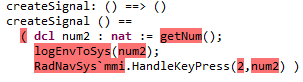
\includegraphics{figures/coverage}
    \caption{Coverage of an operation which has not been
    executed}\label{figure:Coverage} 
\end{figure}

It seems strange that only the first ``('' of the block statement is colored.
It may be more appropriate not to color the parentheses of a block statement at
all. In addition, the \texttt{HandleKeyPress} operation is not colored in red.
This task suggests finding problems with the coverage coloring and improving on
this feature.

\section{Improving robustness of the type checker (PJ)}

Consider the model below with recursive types.

\begin{lstlisting} class A

    types

    public B = C | nat1; public C = B | nat1; 

    end A 
\end{lstlisting}

Using this model we can ask if the union type \texttt{C} is a quote type in the
following way:

\begin{lstlisting} 
    PTypeAssistantTC.isType(C, AQuoteType.class)
\end{lstlisting}

Currently this causes the \texttt{isType} method to call itself recursively
until it fails due to a stack overflow error. This task suggests improving the
\texttt{isType} method to provide robustness for invocations like this.

\section{Improving the Overture debugging features (PJ)}

This task suggests improving debugging in Overture by for instance making it
possible to:

\begin{itemize} 
    \item Set break points that will suspend threads at permission predicates.
    \item Inspect the value of history counters during debugging. 
    \item Use the debugging expression evaluator for all kinds of expressions.  
        \begin{itemize} 
            \item For example, evaluating the expression \texttt{\textbf{dom}
            someMap} currently evaluates to ``set'' instead of actually showing
            what is contained in the set.  
            \item etc.
        \end{itemize} 
\end{itemize}

The documentation example model of the POP3 protocol would serve as a good
starting point for this task.

\section{RT Trace Viewer improvements (PJ)}

When executing a VDM-RT model, a series of events are logged and timestamped by
a component of the Overture tool, called the RT Logger. During execution, these
events are triggered by various actions such as function calls, object
creations and thread activations. These events are logged to a text file and a
binary file with .rt and .rtbin extensions, respectively. The text file can be
inspected by the user using a text editor, while the RT Trace Viewer plugin
enables graphical visualization of the binary trace file. This can be used for
analyzing timing requirements.

This task suggests a series of nice-to-have features and optimization tasks
identified by the plugin authors Martin Askov Andersen, Mads von Qualen and
Peter J\o rgensen:

Suggestions for nice to-have-features: 
\begin{itemize} 
    \item A total overview
        of events for easy scrolling.  
    \item Make ``Move Next'' and ``Move
        Previous'' jump to next/previous visible event instead of ``Next''
        in terms of time.
%\item Auto draw upon resize
    \item The generated conjecture file should be placed in same folder as the
        .rtbin file.  
    \item The generated conjecture file should contain additional information
        which will enable a more precise placement of the conjecture violation
        circle in the RT log viewer. Preferably by supporting the concepts of
        relative time and absolute time like in the NextGen data structure.
        This makes it possible to infer the order of events happening at the
        same point in time. 
    \item Maybe the best solution for conjectures would be to integrate
        the functionality with the NextGen data structure?  
\end{itemize}

Optimizations:

\begin{itemize} 
    \item Change ``jump in time'' model. Currently we draw/parse
        everything for all CPUs when a new time in the future is selected.
        Introduce some sort of history model to save object states when they have
        been parsed. 
    \item Refactor TraceFileRunner to move event-parsing (sorting of
        CPUs etc.) out.  
    \item Refactor eventhandler base to move conjecture handling
        out.  
    \item Cleanup ``update CPU'' hack in TraceFileRunner. 
\end{itemize}

\section{Bug reporting (PJ)}

The current version of Overture lags a feature where users can report bugs.
Such a feature could be available through a \emph{Help} $ \rightarrow$
\emph{Report bug} menu item. This menu item could simply open a browser and
display a web page, where the user could report the bug. Below are some
suggestions for information to add to the bug report:

\begin{itemize} 
    \item A user description of the bug 
    \item Date 
    \item The Overture version 
    \item Log file(s) 
    \item Screen shot(s) 
    \item The VDM project(s) of interest 
    \item etc.  
\end{itemize}




\section{AST-Creator generates documentation (LDC)}

It should be possible to write javadoc content for the nodes of the ast.

ASt creator should be extended in a way that allows users to write the javadoc 
content for each node in seperate files and then point to that documentation in
the main ast definition file.





\chapter{Architecture}


\section{Migration to Interfaces (LDC) } \label{sec:interfacemig}

\subsubsection{The Problem:}

At the moment, various elements used to construct the AST are defined as
classe. For example: \textsf{LexLocation}. When we extend Overture, this
can cause quite a few problems. The COMPASS extensions have slightly
different requirements for these elements so we have to redefine them. But
because we depend on Overture, the original versions are also available to
us. This leads to multiple versions of the same class. Worse, we get the
packages split across multiple bundles (the original versions in the
overture.ide.core bundle and the changed versions in
compassresearch.ide.cml.core bundle). In general, OSGi does not cope very
well with this situaton. In fact, this was the cause of a very problematic
\textsf{java.lang.VerifyError} bug in the COMPASS extension.




\subsubsection{Proposed Solution:}

The elements used to build the AST should be set up as interfaces. Overture
implements its own version of these interfaces and the extensions can
either reuse the Overture classes directly or implement their own versions
as needed.

Ultimately, we should have all the classes in the preamble of the AST
definition file set up as interfaces.

The first step towards this new set up is to define and create interfaces
and convert the existing Overture classes over. LDC has begun this work
when fixing the verify bug. At the moment, only 3 classes have been
converted: \textsf{LexIdentifierToken}, \textsf{LexNameToken} and
\textsf{LexToken}. For the most part, the conversion work isn't very
difficult. Just time consuming, since there are a lot of small errors that
need fixing.





\section{Reorganize Packages (LDC and RL)} The package structure for
Overture is used for internal modularisation which is conflicting with the
scoping mechanisms in Java.  Packages were never intended to be used that
way. The proper way to have internal modularisation is through source
folders.

\begin{sug} 
    Reduce Overture to a few packages with high cohesion. The
    modularisation reflected in existing packages is good but should be realised
    through source folders.  
\end{sug}

With a few well defined packages it becomes feasible to use package-scoping to
create a narrow well scoped interface exposed by the Overture code base.

\begin{sug} 
    Reduce scoping on classes to package scope where possible.
\end{sug}





\section{OSGi Refactoring (LDC and RL)} \label{sec:osgi} 

\subsubsection{The Problem:} Currently, the Overture (and also COMPASS)
OSGi setup is mostly based on the \textsf{Require-Bundle} style. This means
that each bundle imports the whole bundle for everything it needs. Use of
require bundle is generally discouraged \cite{osgi2013}. The recommended
best practice is to use the \textsf{Import-Package} and
\textsf{Export-Package} constructs. Migratation to this style is possible
but would be greatly hindered by the current Overture package structure.


\subsubsection{Proposed Solution:} After reducing the number of packages in
Overture, the manifest files on each project can be changed to use the
package constructs. This work is not particularly complex but will be
rather time consuming since there are many packages that need to be
refactored. Also, these kind of changes have a high potential for conflicts
so special care must be taken with that aspect of the task.







\chapter{Recently Fixed}

\section{Traces}

If you execute traces in the Combinatorial Testing perspective and the test
invokes an operation with a failing precondition the verdict is
\textit{``inconclusive''}. This is how it should be. What seems strange, is
that if you invoke a function with a failing precondition the verdict is
\textit{``failed''}. This task suggests changing this so that functions with
failing preconditions are considered inconclusive as well.

\paragraph{Date:} 21/4-2013.

\paragraph{Solution:} Commit \texttt{271b0ff8785c3d37926238f17a630bdd15138aab}
provides a fix for this.



\begin{thebibliography}{9}

    \bibitem{osgi2013} OSGi Community Wiki, \emph{Require-Bundle}.
        \url{http://wiki.osgi.org/wiki/Require-Bundle}, \emph{Retrieved April 2013}

\end{thebibliography} 

\end{document}
